% !TEX encoding = UTF-8 Unicode
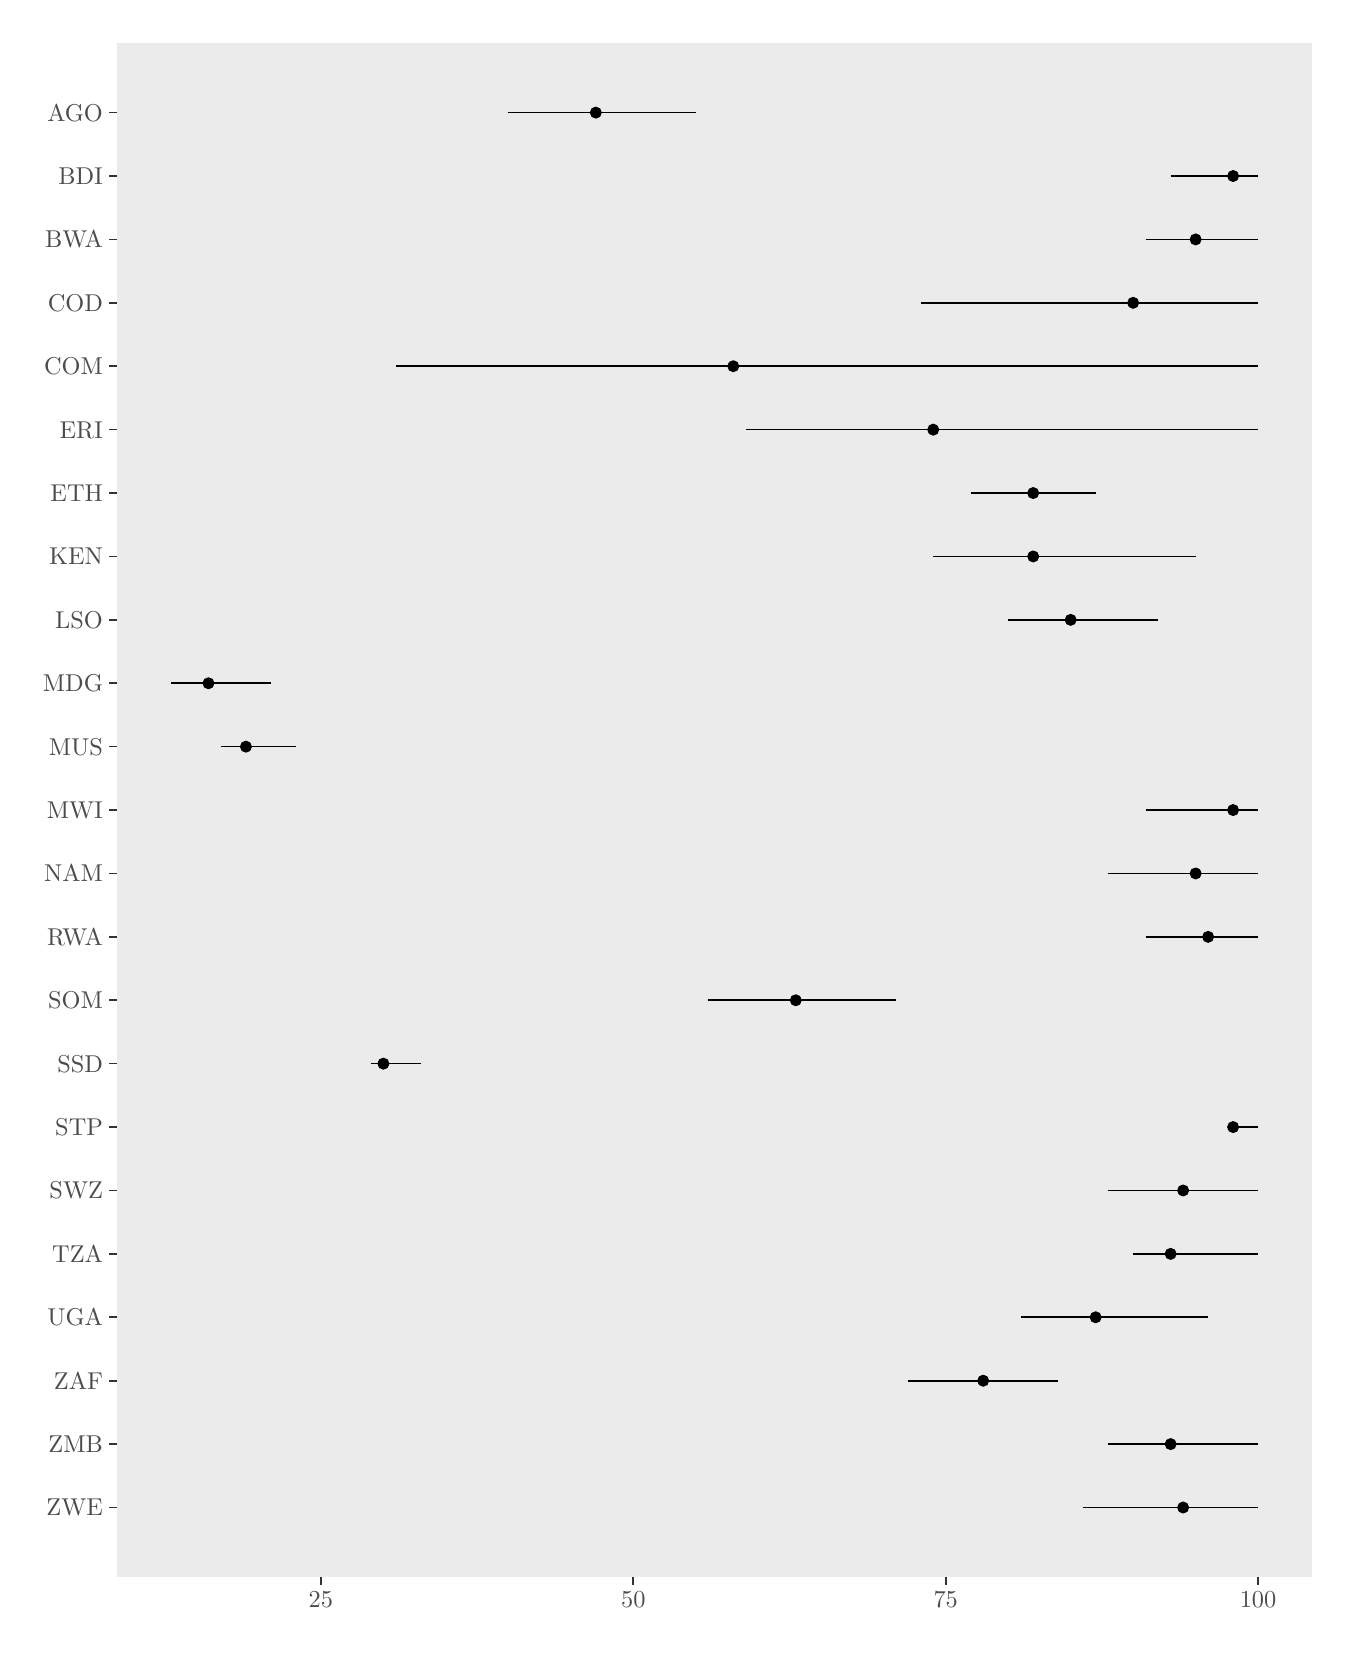
\begin{tikzpicture}[x=1pt,y=1pt]
\definecolor{fillColor}{RGB}{255,255,255}
\path[use as bounding box,fill=fillColor,fill opacity=0.00] (0,0) rectangle (469.75,578.16);
\begin{scope}
\path[clip] (  0.00,  0.00) rectangle (469.75,578.16);
\definecolor{drawColor}{RGB}{255,255,255}
\definecolor{fillColor}{RGB}{255,255,255}

\path[draw=drawColor,line width= 0.6pt,line join=round,line cap=round,fill=fillColor] (  0.00,  0.00) rectangle (469.76,578.16);
\end{scope}
\begin{scope}
\path[clip] ( 32.14, 18.22) rectangle (464.25,572.66);
\definecolor{fillColor}{gray}{0.92}

\path[fill=fillColor] ( 32.14, 18.22) rectangle (464.25,572.66);
\definecolor{drawColor}{RGB}{0,0,0}

\path[draw=drawColor,line width= 0.6pt,line join=round] (173.69,547.46) -- (241.42,547.46);

\path[draw=drawColor,line width= 0.6pt,line join=round] (413.01,524.55) -- (444.61,524.55);

\path[draw=drawColor,line width= 0.6pt,line join=round] (403.98,501.64) -- (444.61,501.64);

\path[draw=drawColor,line width= 0.6pt,line join=round] (322.70,478.73) -- (444.61,478.73);

\path[draw=drawColor,line width= 0.6pt,line join=round] (133.06,455.82) -- (444.61,455.82);

\path[draw=drawColor,line width= 0.6pt,line join=round] (259.49,432.90) -- (444.61,432.90);

\path[draw=drawColor,line width= 0.6pt,line join=round] (340.76,409.99) -- (385.91,409.99);

\path[draw=drawColor,line width= 0.6pt,line join=round] (327.22,387.08) -- (422.04,387.08);

\path[draw=drawColor,line width= 0.6pt,line join=round] (354.31,364.17) -- (408.49,364.17);

\path[draw=drawColor,line width= 0.6pt,line join=round] ( 51.78,341.26) -- ( 87.90,341.26);

\path[draw=drawColor,line width= 0.6pt,line join=round] ( 69.84,318.35) -- ( 96.93,318.35);

\path[draw=drawColor,line width= 0.6pt,line join=round] (403.98,295.44) -- (444.61,295.44);

\path[draw=drawColor,line width= 0.6pt,line join=round] (390.43,272.53) -- (444.61,272.53);

\path[draw=drawColor,line width= 0.6pt,line join=round] (403.98,249.62) -- (444.61,249.62);

\path[draw=drawColor,line width= 0.6pt,line join=round] (245.94,226.71) -- (313.67,226.71);

\path[draw=drawColor,line width= 0.6pt,line join=round] (124.03,203.80) -- (142.09,203.80);

\path[draw=drawColor,line width= 0.6pt,line join=round] (435.58,180.89) -- (444.61,180.89);

\path[draw=drawColor,line width= 0.6pt,line join=round] (390.43,157.98) -- (444.61,157.98);

\path[draw=drawColor,line width= 0.6pt,line join=round] (399.46,135.07) -- (444.61,135.07);

\path[draw=drawColor,line width= 0.6pt,line join=round] (358.82,112.16) -- (426.55,112.16);

\path[draw=drawColor,line width= 0.6pt,line join=round] (318.18, 89.24) -- (372.37, 89.24);

\path[draw=drawColor,line width= 0.6pt,line join=round] (390.43, 66.33) -- (444.61, 66.33);

\path[draw=drawColor,line width= 0.6pt,line join=round] (381.40, 43.42) -- (444.61, 43.42);
\definecolor{fillColor}{RGB}{0,0,0}

\path[draw=drawColor,line width= 0.4pt,line join=round,line cap=round,fill=fillColor] (205.30,547.46) circle (  1.96);

\path[draw=drawColor,line width= 0.4pt,line join=round,line cap=round,fill=fillColor] (435.58,524.55) circle (  1.96);

\path[draw=drawColor,line width= 0.4pt,line join=round,line cap=round,fill=fillColor] (422.04,501.64) circle (  1.96);

\path[draw=drawColor,line width= 0.4pt,line join=round,line cap=round,fill=fillColor] (399.46,478.73) circle (  1.96);

\path[draw=drawColor,line width= 0.4pt,line join=round,line cap=round,fill=fillColor] (254.97,455.82) circle (  1.96);

\path[draw=drawColor,line width= 0.4pt,line join=round,line cap=round,fill=fillColor] (327.22,432.90) circle (  1.96);

\path[draw=drawColor,line width= 0.4pt,line join=round,line cap=round,fill=fillColor] (363.34,409.99) circle (  1.96);

\path[draw=drawColor,line width= 0.4pt,line join=round,line cap=round,fill=fillColor] (363.34,387.08) circle (  1.96);

\path[draw=drawColor,line width= 0.4pt,line join=round,line cap=round,fill=fillColor] (376.88,364.17) circle (  1.96);

\path[draw=drawColor,line width= 0.4pt,line join=round,line cap=round,fill=fillColor] ( 65.33,341.26) circle (  1.96);

\path[draw=drawColor,line width= 0.4pt,line join=round,line cap=round,fill=fillColor] ( 78.87,318.35) circle (  1.96);

\path[draw=drawColor,line width= 0.4pt,line join=round,line cap=round,fill=fillColor] (435.58,295.44) circle (  1.96);

\path[draw=drawColor,line width= 0.4pt,line join=round,line cap=round,fill=fillColor] (422.04,272.53) circle (  1.96);

\path[draw=drawColor,line width= 0.4pt,line join=round,line cap=round,fill=fillColor] (426.55,249.62) circle (  1.96);

\path[draw=drawColor,line width= 0.4pt,line join=round,line cap=round,fill=fillColor] (277.55,226.71) circle (  1.96);

\path[draw=drawColor,line width= 0.4pt,line join=round,line cap=round,fill=fillColor] (128.54,203.80) circle (  1.96);

\path[draw=drawColor,line width= 0.4pt,line join=round,line cap=round,fill=fillColor] (435.58,180.89) circle (  1.96);

\path[draw=drawColor,line width= 0.4pt,line join=round,line cap=round,fill=fillColor] (417.52,157.98) circle (  1.96);

\path[draw=drawColor,line width= 0.4pt,line join=round,line cap=round,fill=fillColor] (413.01,135.07) circle (  1.96);

\path[draw=drawColor,line width= 0.4pt,line join=round,line cap=round,fill=fillColor] (385.91,112.16) circle (  1.96);

\path[draw=drawColor,line width= 0.4pt,line join=round,line cap=round,fill=fillColor] (345.28, 89.24) circle (  1.96);

\path[draw=drawColor,line width= 0.4pt,line join=round,line cap=round,fill=fillColor] (413.01, 66.33) circle (  1.96);

\path[draw=drawColor,line width= 0.4pt,line join=round,line cap=round,fill=fillColor] (417.52, 43.42) circle (  1.96);
\end{scope}
\begin{scope}
\path[clip] (  0.00,  0.00) rectangle (469.75,578.16);
\definecolor{drawColor}{gray}{0.30}

\node[text=drawColor,anchor=base east,inner sep=0pt, outer sep=0pt, scale=  0.88] at ( 27.19,544.43) {AGO};

\node[text=drawColor,anchor=base east,inner sep=0pt, outer sep=0pt, scale=  0.88] at ( 27.19,521.52) {BDI};

\node[text=drawColor,anchor=base east,inner sep=0pt, outer sep=0pt, scale=  0.88] at ( 27.19,498.61) {BWA};

\node[text=drawColor,anchor=base east,inner sep=0pt, outer sep=0pt, scale=  0.88] at ( 27.19,475.70) {COD};

\node[text=drawColor,anchor=base east,inner sep=0pt, outer sep=0pt, scale=  0.88] at ( 27.19,452.79) {COM};

\node[text=drawColor,anchor=base east,inner sep=0pt, outer sep=0pt, scale=  0.88] at ( 27.19,429.87) {ERI};

\node[text=drawColor,anchor=base east,inner sep=0pt, outer sep=0pt, scale=  0.88] at ( 27.19,406.96) {ETH};

\node[text=drawColor,anchor=base east,inner sep=0pt, outer sep=0pt, scale=  0.88] at ( 27.19,384.05) {KEN};

\node[text=drawColor,anchor=base east,inner sep=0pt, outer sep=0pt, scale=  0.88] at ( 27.19,361.14) {LSO};

\node[text=drawColor,anchor=base east,inner sep=0pt, outer sep=0pt, scale=  0.88] at ( 27.19,338.23) {MDG};

\node[text=drawColor,anchor=base east,inner sep=0pt, outer sep=0pt, scale=  0.88] at ( 27.19,315.32) {MUS};

\node[text=drawColor,anchor=base east,inner sep=0pt, outer sep=0pt, scale=  0.88] at ( 27.19,292.41) {MWI};

\node[text=drawColor,anchor=base east,inner sep=0pt, outer sep=0pt, scale=  0.88] at ( 27.19,269.50) {NAM};

\node[text=drawColor,anchor=base east,inner sep=0pt, outer sep=0pt, scale=  0.88] at ( 27.19,246.59) {RWA};

\node[text=drawColor,anchor=base east,inner sep=0pt, outer sep=0pt, scale=  0.88] at ( 27.19,223.68) {SOM};

\node[text=drawColor,anchor=base east,inner sep=0pt, outer sep=0pt, scale=  0.88] at ( 27.19,200.77) {SSD};

\node[text=drawColor,anchor=base east,inner sep=0pt, outer sep=0pt, scale=  0.88] at ( 27.19,177.86) {STP};

\node[text=drawColor,anchor=base east,inner sep=0pt, outer sep=0pt, scale=  0.88] at ( 27.19,154.95) {SWZ};

\node[text=drawColor,anchor=base east,inner sep=0pt, outer sep=0pt, scale=  0.88] at ( 27.19,132.04) {TZA};

\node[text=drawColor,anchor=base east,inner sep=0pt, outer sep=0pt, scale=  0.88] at ( 27.19,109.12) {UGA};

\node[text=drawColor,anchor=base east,inner sep=0pt, outer sep=0pt, scale=  0.88] at ( 27.19, 86.21) {ZAF};

\node[text=drawColor,anchor=base east,inner sep=0pt, outer sep=0pt, scale=  0.88] at ( 27.19, 63.30) {ZMB};

\node[text=drawColor,anchor=base east,inner sep=0pt, outer sep=0pt, scale=  0.88] at ( 27.19, 40.39) {ZWE};
\end{scope}
\begin{scope}
\path[clip] (  0.00,  0.00) rectangle (469.75,578.16);
\definecolor{drawColor}{gray}{0.20}

\path[draw=drawColor,line width= 0.6pt,line join=round] ( 29.39,547.46) --
	( 32.14,547.46);

\path[draw=drawColor,line width= 0.6pt,line join=round] ( 29.39,524.55) --
	( 32.14,524.55);

\path[draw=drawColor,line width= 0.6pt,line join=round] ( 29.39,501.64) --
	( 32.14,501.64);

\path[draw=drawColor,line width= 0.6pt,line join=round] ( 29.39,478.73) --
	( 32.14,478.73);

\path[draw=drawColor,line width= 0.6pt,line join=round] ( 29.39,455.82) --
	( 32.14,455.82);

\path[draw=drawColor,line width= 0.6pt,line join=round] ( 29.39,432.90) --
	( 32.14,432.90);

\path[draw=drawColor,line width= 0.6pt,line join=round] ( 29.39,409.99) --
	( 32.14,409.99);

\path[draw=drawColor,line width= 0.6pt,line join=round] ( 29.39,387.08) --
	( 32.14,387.08);

\path[draw=drawColor,line width= 0.6pt,line join=round] ( 29.39,364.17) --
	( 32.14,364.17);

\path[draw=drawColor,line width= 0.6pt,line join=round] ( 29.39,341.26) --
	( 32.14,341.26);

\path[draw=drawColor,line width= 0.6pt,line join=round] ( 29.39,318.35) --
	( 32.14,318.35);

\path[draw=drawColor,line width= 0.6pt,line join=round] ( 29.39,295.44) --
	( 32.14,295.44);

\path[draw=drawColor,line width= 0.6pt,line join=round] ( 29.39,272.53) --
	( 32.14,272.53);

\path[draw=drawColor,line width= 0.6pt,line join=round] ( 29.39,249.62) --
	( 32.14,249.62);

\path[draw=drawColor,line width= 0.6pt,line join=round] ( 29.39,226.71) --
	( 32.14,226.71);

\path[draw=drawColor,line width= 0.6pt,line join=round] ( 29.39,203.80) --
	( 32.14,203.80);

\path[draw=drawColor,line width= 0.6pt,line join=round] ( 29.39,180.89) --
	( 32.14,180.89);

\path[draw=drawColor,line width= 0.6pt,line join=round] ( 29.39,157.98) --
	( 32.14,157.98);

\path[draw=drawColor,line width= 0.6pt,line join=round] ( 29.39,135.07) --
	( 32.14,135.07);

\path[draw=drawColor,line width= 0.6pt,line join=round] ( 29.39,112.16) --
	( 32.14,112.16);

\path[draw=drawColor,line width= 0.6pt,line join=round] ( 29.39, 89.24) --
	( 32.14, 89.24);

\path[draw=drawColor,line width= 0.6pt,line join=round] ( 29.39, 66.33) --
	( 32.14, 66.33);

\path[draw=drawColor,line width= 0.6pt,line join=round] ( 29.39, 43.42) --
	( 32.14, 43.42);
\end{scope}
\begin{scope}
\path[clip] (  0.00,  0.00) rectangle (469.75,578.16);
\definecolor{drawColor}{gray}{0.20}

\path[draw=drawColor,line width= 0.6pt,line join=round] (105.96, 15.47) --
	(105.96, 18.22);

\path[draw=drawColor,line width= 0.6pt,line join=round] (218.85, 15.47) --
	(218.85, 18.22);

\path[draw=drawColor,line width= 0.6pt,line join=round] (331.73, 15.47) --
	(331.73, 18.22);

\path[draw=drawColor,line width= 0.6pt,line join=round] (444.61, 15.47) --
	(444.61, 18.22);
\end{scope}
\begin{scope}
\path[clip] (  0.00,  0.00) rectangle (469.75,578.16);
\definecolor{drawColor}{gray}{0.30}

\node[text=drawColor,anchor=base,inner sep=0pt, outer sep=0pt, scale=  0.88] at (105.96,  7.21) {25};

\node[text=drawColor,anchor=base,inner sep=0pt, outer sep=0pt, scale=  0.88] at (218.85,  7.21) {50};

\node[text=drawColor,anchor=base,inner sep=0pt, outer sep=0pt, scale=  0.88] at (331.73,  7.21) {75};

\node[text=drawColor,anchor=base,inner sep=0pt, outer sep=0pt, scale=  0.88] at (444.61,  7.21) {100};
\end{scope}
\end{tikzpicture}
